\documentclass[aspectratio=169]{beamer}

% --- Packages ---
\usepackage{amsfonts,amsmath,oldgerm,algorithm,algpseudocode}
\usepackage[font=small,labelfont=bf]{caption}
\usepackage{animate}
\usepackage{tikz}
\usepackage{listings}
\usepackage[most]{tcolorbox}
\usetikzlibrary{calc, positioning}

% Hand-made artwork lives in assets/; every data figure is regenerated into
% figures/ by make_slide_figures.py (see build.sh).
\graphicspath{{figures/}{assets/}}

% --- Color Palette ---
\definecolor{bluegray}{HTML}{8d99ae} %medium blue-gray
\definecolor{lightgray}{HTML}{edf2f4} % Background for blocks/listings
\definecolor{darkgray}{HTML}{2b2d42} % Navy/Dark Gray
\definecolor{sectionbox}{HTML}{303861} % Slightly lighter shade of darkgray

% --- Typography & Alignment ---
\usefonttheme[onlymath]{serif}
\setbeamercolor{normal text}{fg=black}

% Align all body text perfectly with the title offset (1.5cm)
\setbeamersize{text margin left=1.5cm, text margin right=1.5cm}

% --- Presentation Metadata ---
\title{Optical Turbulence in the Ikeda Map}
\subtitle{\textbf{High-Performance Computing \\ and Chaos Theory}}
\author{Rahul Nivash}
\date{Theory Canada \textbullet\ June 20, 2026}

% ==========================================
% TEMPLATE CUSTOMIZATIONS
% ==========================================

% 1. Disable Navigation Symbols
\setbeamertemplate{navigation symbols}{}

% 2. Title Page Design
\setbeamertemplate{title page}{
    \begin{tikzpicture}[remember picture,overlay]
        % Draw the dark gray background directly
        \fill[darkgray] (current page.north west) rectangle (current page.south east);
        
        % Left side white overlay with diagonal cut
        \fill[white] (current page.north west) -- (current page.south west) -- 
                     ([xshift=7.5cm]current page.south west) -- 
                     ([xshift=10cm]current page.north west) -- cycle;

        % Title Text Layout 
        \node[anchor=west, text=darkgray, font=\huge\bfseries, align=left, text width=8cm, inner xsep=0pt] 
            at ([xshift=1.1cm, yshift=2.6cm]current page.west) {\inserttitle};
            
        \node[anchor=west, text=bluegray, font=\Large, align=left, text width=8cm, inner xsep=0pt] 
            at ([xshift=1.1cm, yshift=0.8cm]current page.west) {\insertsubtitle};
            
        % Divider Line
        \draw[thick] ([xshift=1.1cm, yshift=-0.1cm]current page.west) -- ([xshift=8cm, yshift=-0.1cm]current page.west);
        
        % Meta Data
        \node[anchor=west, text=darkgray, font=\large, inner xsep=0pt] 
            at ([xshift=1.1cm, yshift=-0.7cm]current page.west) {\insertauthor};
            
        \node[anchor=west, text=bluegray, font=\small\bfseries, inner xsep=0pt] 
            at ([xshift=1.1cm, yshift=-1.3cm]current page.west) {\insertdate};
            
        % University logo
        \node[anchor=west, inner sep=0pt] 
            at ([xshift=1.1cm, yshift=-2.7cm]current page.west) {
            
\includegraphics[height=1.5cm]{logo.jpg} 
        };
        
        % Bifurcation cascade on the dark right-hand side (figures/ikeda_cascade.png)
        \node[anchor=east, inner sep=0pt] 
            at (current page.east) {
            \includegraphics[width=6.5cm]{ikeda_cascade.png} 
        };
        
    \end{tikzpicture}
}
% 3. Frame Title Design
\setbeamertemplate{frametitle}{
    \vspace{0.4cm} 
    \begin{tikzpicture}[remember picture,overlay]
        % Section Number Box
        \node[anchor=north west, fill=sectionbox, text=white, minimum width=1.3cm, minimum height=1.3cm, font=\Large\bfseries, inner sep=0pt] 
            at (current page.north west) {\S\thesection};
            
        % Frame Title & Subtitle Layout
        \node[anchor=west, text=darkgray, align=left, inner xsep=0pt] 
            at ([xshift=1.5cm, yshift=-0.65cm]current page.north west) {
                {\Large\bfseries \insertframetitle}
                \ifx\insertframesubtitle\@empty\else\\[-0.05cm]
                {\normalsize\bfseries\color{bluegray}\insertframesubtitle}\fi
            };
    \end{tikzpicture}
    \vspace{0.4cm} 
}

% 4. Footer Design (Progress Bar + Section Text + Static Number)
\setbeamertemplate{footline}{
    \begin{tikzpicture}[remember picture,overlay]
        % Calculate progress percentage
        \ifnum\inserttotalframenumber>0
            \pgfmathsetmacro{\progress}{\insertframenumber/\inserttotalframenumber}
        \else
            \pgfmathsetmacro{\progress}{0}
        \fi
        
        % Define coordinates aligned exactly with text margins
        \coordinate (Start) at ([xshift=1.5cm, yshift=0.6cm]current page.south west);
        \coordinate (End) at ([xshift=-1.5cm, yshift=0.6cm]current page.south east);
        
        % Draw faint track line
        \draw[draw=black!15, thick] (Start) -- (End);
        
        % Draw active progress bar
        \draw[draw=darkgray, thick] (Start) -- ($ (Start) ! \progress ! (End) $);
        
        % Place the section text just below the start of the progress bar
        \node[anchor=north west, font=\scriptsize\bfseries, text=darkgray, inner sep=0pt] 
            at ([yshift=-0.15cm]Start) {Section \thesection: \insertsection};
        
        % Place the static slide number at the far right edge
        \node[anchor=west, font=\small, text=black, inner sep=0pt] 
            at ([xshift=0.3cm]End) {\insertframenumber};
    \end{tikzpicture}
}
% 1. Preamble setup
\newcommand{\sectionimg}{} % Default is empty
\newcommand{\setsectionimage}[1]{\renewcommand{\sectionimg}{#1}}

% 2. Updated Divider Template
\AtBeginSection[]{
    \begin{frame}[plain]
        \begin{tikzpicture}[remember picture,overlay]
            \fill[white] (current page.north west) rectangle (current page.south east);
            \fill[darkgray] (current page.north west) -- (current page.south west) -- 
                            ([xshift=10cm]current page.south west) -- 
                            ([xshift=6cm]current page.north west) -- cycle;

            \node[anchor=west, text=bluegray, font=\Large\bfseries, inner xsep=0pt] 
                at ([xshift=1.5cm, yshift=0.5cm]current page.west) {Part \thesection};
            \node[anchor=west, text=white, font=\huge\bfseries, align=left, inner xsep=0pt] (sectitle)
                at ([xshift=1.5cm, yshift=-0.2cm]current page.west) {\insertsection};
                
            \coordinate (LineStart) at ([xshift=1.5cm, yshift=-0.7cm]current page.west);
            \coordinate (LineEnd) at ([xshift=0.04cm]sectitle.south east |- LineStart);
            \draw[thick, draw=bluegray] (LineStart) -- (LineEnd);
            
            % --- CONDITIONAL IMAGE LOGIC ---
            \ifx\sectionimg\empty\else
                \node[anchor=east, inner sep=0pt] at ([xshift=-1cm]current page.east) {
                    \includegraphics[width=5cm, keepaspectratio]{\sectionimg} 
                };
            \fi
        \end{tikzpicture}
    \end{frame}
}
% 5. Itemize Design
\setbeamertemplate{itemize item}{\color{bluegray}\rule{1ex}{1ex}}
\setbeamertemplate{itemize subitem}{\color{bluegray}\rule{0.8ex}{0.8ex}}
\setbeamertemplate{itemize subsubitem}{\color{bluegray}\rule{0.6ex}{0.6ex}}
\setlength{\leftmargini}{1em} 

% 6. Listings Styling
\lstset{
    backgroundcolor=\color{lightgray},
    basicstyle=\ttfamily\small,
    numbers=left,
    numberstyle=\tiny\color{darkgray},
    frame=tb, 
    rulecolor=\color{black},
    xleftmargin=0pt, 
    framexleftmargin=0pt,
    aboveskip=1em,
    belowskip=1em
}

% 7. Custom Block Environments
\newtcolorbox{customblock}[1]{
    enhanced, sharp corners, boxrule=0pt, colback=lightgray, 
    borderline west={4pt}{0pt}{bluegray},
    title=#1, coltitle=white, colbacktitle=bluegray,
    attach boxed title to top left={yshift=0mm, xshift=0mm},
    boxed title style={sharp corners, boxrule=0pt}, 
    top=4mm, bottom=2mm,
    left=2mm, right=2mm,
    boxsep=2mm
}

\begin{document}

% --- Title ---
\begin{frame}[plain]
    \titlepage
\end{frame}

\setsectionimage{ringtitle.png}
\section{Introduction}
\begin{frame}{The Nonlinear Optical Ring Cavity}{Physical Dynamics}
    \begin{columns}[T, onlytextwidth]
        
        % Left Column: The Schematic Diagram
        \begin{column}{0.45\textwidth}
            \vspace{0pt} % Aligns top of image with top of right column
            \centering
            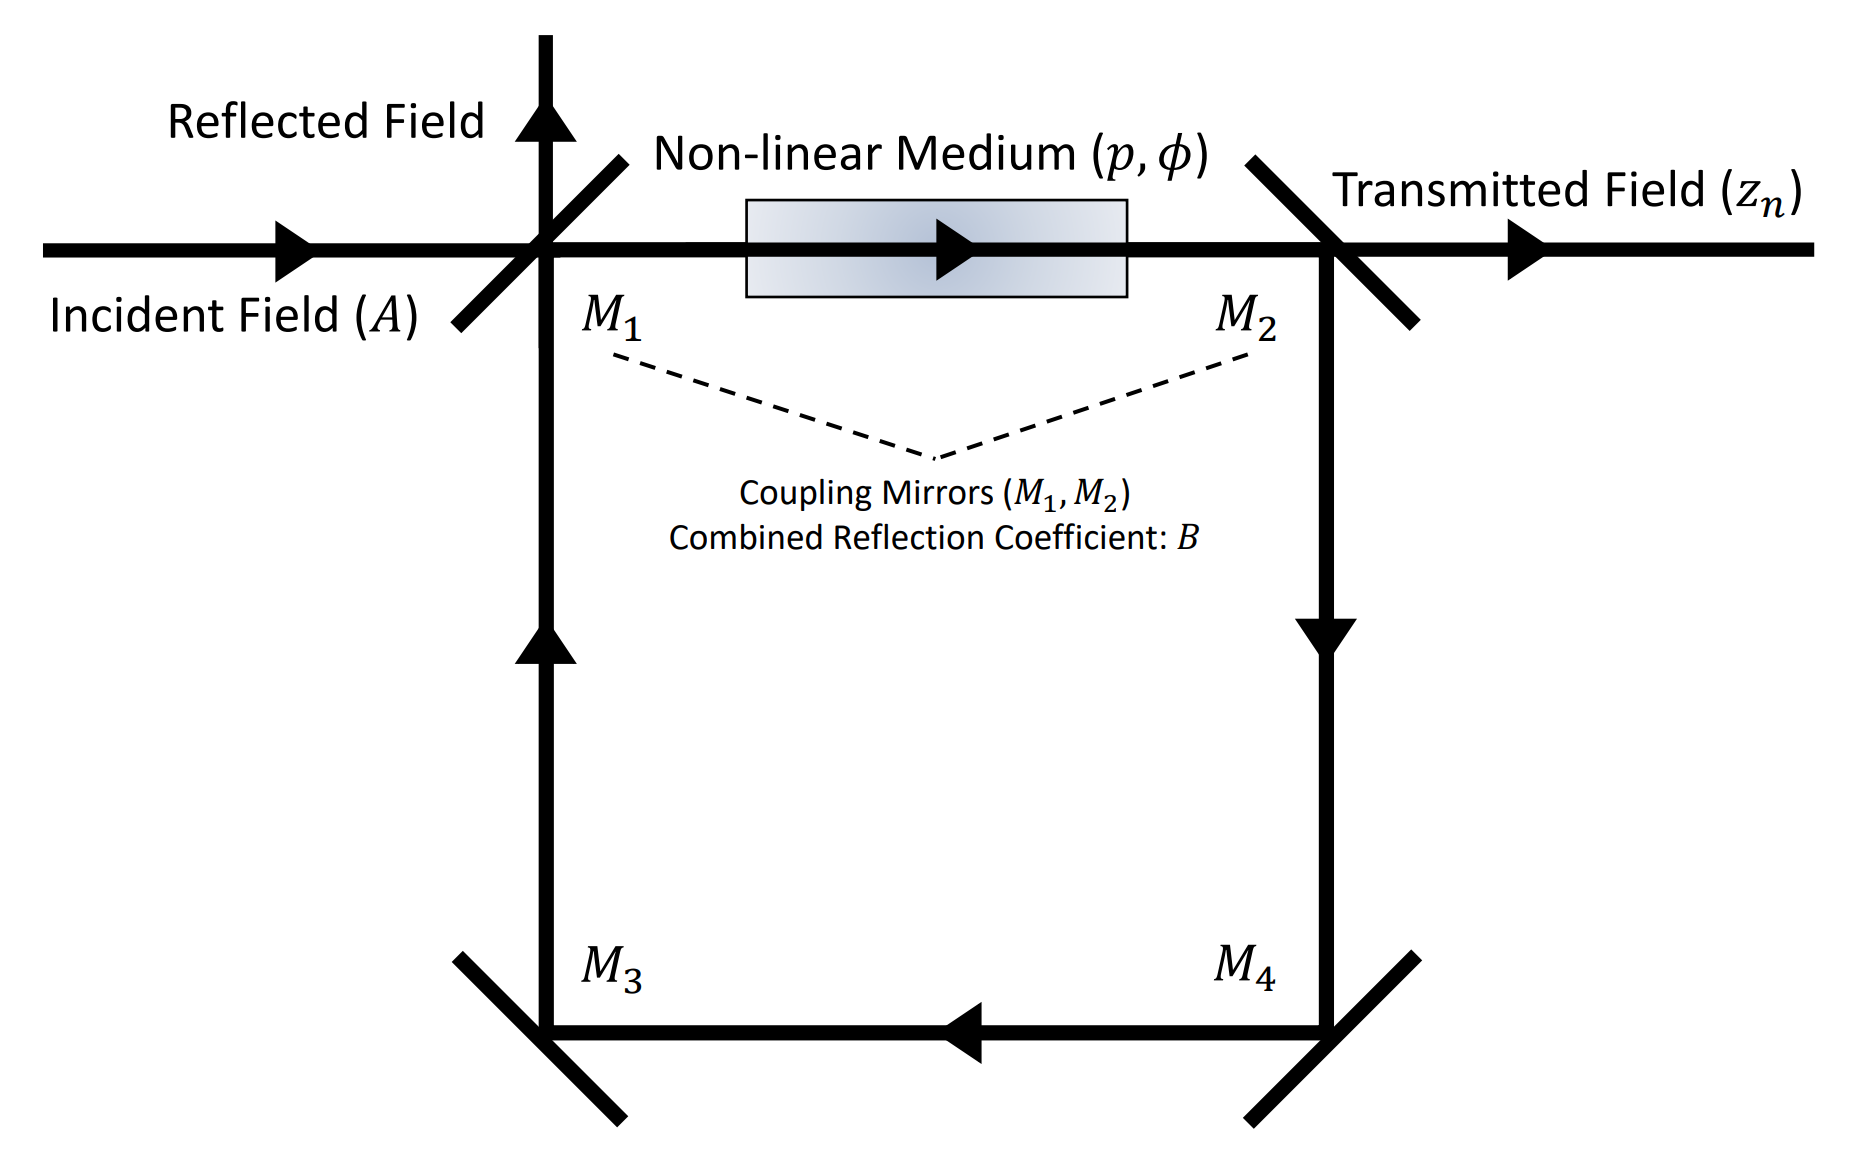
\includegraphics[width=\textwidth]{ring_cavity.png}
            \\[2pt] % Small vertical space before caption
            {\footnotesize \textit{Unidirectional nonlinear ring cavity.}}
        \end{column}
        
        % Right Column: Physical Mechanism Summary
        \begin{column}{0.52\textwidth}      
            \vspace{0pt} % Ensures top alignment with left column
            \begin{itemize}
                \item Light circulating within a non-linear ring cavity can exhibit chaotic fluctuations, a phenomenon known as optical turbulence.
                
                \item The electromagnetic field experiences feedback at distinct intervals upon reflecting off the cavity mirrors.
                
                \item This feedback requires an iterative map to capture the dynamical instabilities.
            \end{itemize}
        \end{column}
        
    \end{columns}
\end{frame}

% --- The Physical Paradigm ---
\begin{frame}{The Nonlinear Optical Ring Cavity}{Historical Context}
    \begin{columns}[T, onlytextwidth]
        
        % Column 1: The Historical Standard
        \begin{column}{0.48\textwidth}
            \textbf{Conventional CW Theories}
            \begin{itemize}
                \item Standard for modeling optical bistability prior to 1979.
                \item Assumed continuous phase space evolution.
                \item Failed to capture dynamical instabilities arising from feedback delay.
            \end{itemize}
        \end{column}
        
        % Column 2: The Ikeda Paradigm
        \begin{column}{0.48\textwidth}
            \textbf{Ikeda's Prediction (1979)}
            \begin{itemize}
                \item Proposed discrete-time iterative maps; i.e. $z_{n+1} = f(z_n)$.
                \item Predicted chaotic fluctuations (optical turbulence) due to round-trip delay.
                \item Shifted focus from stationary states to dynamic evolution.
            \end{itemize}
        \end{column}
        
    \end{columns}

    \vspace{1em}
    
\end{frame}



% --- Mathematical Formulation ---
\begin{frame}{The Nonlinear Optical Ring Cavity}{The Ikeda Map}
    \vspace{-3.5em}
\begin{block}{}
        \centering
        $z_{n+1} = A + B z_n \exp\left[i\left(\phi - \frac{p}{1+|z_n|^2}\right)\right]$
\end{block}
    \vspace{1.5em}
    \textbf{Definition of Parameters:}
    \begin{itemize}
        \item \textbf{$z_n \in \mathbb{C}$}: Transmitted electric field at the $n$-th
        iteration.
        \item \textbf{$A$}: Amplitude of the input light injected into the ring cavity.
        \item \textbf{$B$}: Reflection coefficient of the cavity mirrors.
        \item \textbf{$\phi$}: Linear phase shift.
        \item \textbf{$p$}: Nonlinear phase shift.
    \end{itemize}
    
    \vspace{0.5em}
\end{frame}

\setsectionimage{nvidia-cuda_logo.png}
\section{HPC Architecture}
% --- The Iterative Burden ---
\begin{frame}[t]{Computational Bottlenecks}{The Cost of Simulating Chaos}
    
    Modeling optical turbulence requires massive computational resources:
    
    % Top Block: The generation problem
    \begin{customblock}{1. The Iterative Burden}
        \begin{itemize}
            \item \textbf{Complex Arithmetic:} Every iteration evaluates a complex exponential of a field-dependent phase.
            
            \item \textbf{High-Resolution Sweeps:} To observe the route to chaos, the simulation evaluates thousands to millions of reflection coefficients ($B$), each for thousands of round trips.
        \end{itemize}
    \end{customblock}
    
    % Bottom Metric Graphic
    \vspace{0cm}
    \begin{center}
        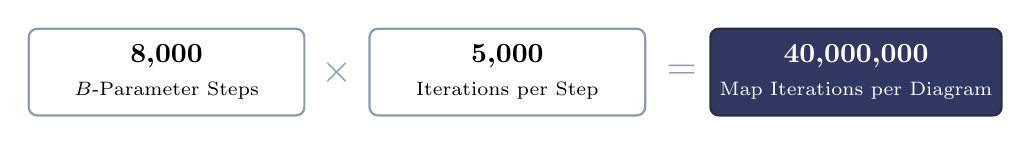
\begin{tikzpicture}[
            statbox/.style={rectangle, rounded corners=3pt, fill=white, draw=bluegray, thick, minimum width=3.5cm, minimum height=1.1cm, align=center},
            arrow/.style={->, >=stealth, thick, draw=bluegray}
        ]
            % Nodes
            \node[statbox] (bvals) {\textbf{8,000} \\ \scriptsize $B$-Parameter Steps};
            \node[statbox, right=0.8cm of bvals] (iters) {\textbf{5,000} \\ \scriptsize Iterations per Step};
            
            % Highlighted Result Node
            \node[statbox, right=0.8cm of iters, fill=sectionbox, text=white, draw=darkgray] (total) {\textbf{40,000,000} \\ \scriptsize Map Iterations per Diagram};
            
            % Connecting Math Symbols
            \node[font=\Large\bfseries\color{bluegray}] at ($(bvals)!0.5!(iters)$) {$\times$};
            \node[font=\Large\bfseries\color{bluegray}] at ($(iters)!0.5!(total)$) {$=$};
        \end{tikzpicture}
    \end{center}
    
\end{frame}

% --- Quantification Overhead ---
\begin{frame}[t]{Computational Bottlenecks}{The Cost of Simulating Chaos}
    
    Modeling optical turbulence requires massive computational resources:
    
    % Bottom Block: The analysis problem
    \begin{customblock}{2. Quantification Overhead}
        \begin{itemize}
            \item \textbf{Lyapunov Exponents:} Confirming chaos requires calculating the $2\times2$ Jacobian matrix at every iteration step.
            
            \item \textbf{Fractal Dimensions:} Quantifying geometry of the attractor requires box-counting algorithms to repeatedly scan the entire phase space.
            
            \item \textbf{Stability Extraction:} Locating limits of the bifurcation cascade requires multi-dimensional root-finding methods.
        \end{itemize}
    \end{customblock}
    
\end{frame}
% --- The Baseline Algorithm ---
\begin{frame}[fragile, c]{Baseline Simulation}{The Complex Iteration Algorithm}
    \vspace{-3em}
    \begin{algorithm}[H]
    \fontsize{8}{1.1}\selectfont
    \caption{Complex Ikeda Map Simulation}
    \begin{algorithmic}[1]
        \Require \textbf{Input:} Target bounds ($B_{\text{start}}, B_{\text{end}}, B_{\text{steps}}$)
        \Require \textbf{Parameters:} Input amplitude $A$, phase shift $\phi$, nonlinear parameter $p$
        \Require \textbf{Lengths:} $N_{\text{transient}}$ (discard phase), $N_{\text{record}}$ (steady-state)
        \Ensure \textbf{Output:} Array of asymptotic steady-state amplitudes $|z|$ mapped to $B$
        
        \vspace{0.1cm}
        \ForAll{$B \in B\_values$ \textbf{in parallel across GPU threads}}
            \State $z \leftarrow 0 + 0i$ \Comment{Initial condition}
            
            \For{$j \leftarrow 1 \text{ to } (N_{transient} + N_{record})$}
                \State $z \leftarrow A + B \cdot z \cdot \exp\left[i\left(\phi - \frac{p}{1 + |z|^2}\right)\right]$
                
                \If{$j > N_{transient}$}
                    \State Save $|z|$ mapped to thread index $B$
                \EndIf
            \EndFor
        \EndFor
    \end{algorithmic}
    \end{algorithm}
\end{frame}

% --- Visualizing the Hardware Difference ---
\begin{frame}{High-Performance Computing}{CPU vs. GPU Architectures}
    \begin{center}
        % Syntax: \animategraphics[options]{framerate}{file_prefix}{start_frame}{end_frame}
        % The 'loop' and 'controls' options add play/pause buttons (Adobe Reader / Okular).
        \animategraphics[loop, controls, width=0.85\textwidth]{24}{figures/animation/frame_}{000}{119}
    \end{center}
\end{frame}

% --- 2D Decoupled Mapping ---
\begin{frame}{2D Decoupled Architecture}{Optimizing the Ikeda Map}
    \begin{columns}[T, onlytextwidth]
        
        % Left Column: The Equations
        \begin{column}{0.55\textwidth}
            \vspace*{-0.9cm} % Shifts the entire left column up closer to the title
            
            \begin{customblock}{Original Complex Map}
                \vspace{-0.2cm} % Compresses the block's internal top padding
                \centering
                \resizebox{0.95\linewidth}{!}{$\displaystyle z_{n+1} = A + B z_n \exp\left[ i \left( \phi - \frac{p}{1 + |z_n|^2} \right) \right]$}
            \end{customblock}
            
            \vspace*{-0.15cm} % Pulls the second box tighter to the first box
            
            \begin{customblock}{2D Real-Valued Map}
                \vspace{-0.2cm} % Compresses the block's internal top padding
                \centering
                $\begin{aligned}
                    x_{n+1} &= A + B(x_n \cos t_n - y_n \sin t_n) \\
                    y_{n+1} &= B(x_n \sin t_n + y_n \cos t_n) \\
                    t_n &= \phi - \frac{p}{x_n^2 + y_n^2 + 1}
                \end{aligned}$
            \end{customblock}
            
        \end{column}
        
% Right Column: Impact
        \begin{column}{0.38\textwidth}
                    \vspace*{-0.7cm} % Shifts the entire left column up closer to the title

            \begin{itemize}
                \item \textbf{No Complex Arithmetic:} One \texttt{sincos} and a few multiply-adds per round trip.
                
                \item \textbf{Closed-Form Jacobian:} Lyapunov exponents for $\sim$10 extra FLOPs per step; $\det J = B^2$.
                
                \item \textbf{One Thread per $B$:} Independent orbits, no locks, and coalesced memory writes.
            \end{itemize}

        \end{column}
        
    \end{columns}
\end{frame}

% --- The Optimized Algorithm ---
\begin{frame}[fragile, c]{Optimized Simulation}{The 2D Decoupled Algorithm}
    \vspace{-2em}
    \begin{algorithm}[H]
    \fontsize{8}{1.1}\selectfont
    \caption{Decoupled Ikeda Map Simulation}
    \begin{algorithmic}[1]
        \Require \textbf{Input:} Target bounds ($B_{\text{start}}, B_{\text{end}}, B_{\text{steps}}$)
        \Require \textbf{Parameters:} Input amplitude $A$, phase shift $\phi$, nonlinear parameter $p$
        \Require \textbf{Lengths:} $N_{\text{transient}}$ (discard phase), $N_{\text{record}}$ (steady-state)
        \Ensure \textbf{Output:} Arrays of steady-state coordinates $(x, y)$ and amplitudes mapped to $B$
        
        \ForAll{$B \in B\_values$ \textbf{in parallel across GPU threads}}
            \State $x \leftarrow 0, y \leftarrow 0$ \Comment{Initial condition}
            
            \For{$j \leftarrow 1 \text{ to } (N_{transient} + N_{record})$}
                \State $t_n \leftarrow \phi - \frac{p}{x^2 + y^2 + 1}$
                \State $x_{new} \leftarrow A + B(x \cos t_n - y \sin t_n)$
                \State $y_{new} \leftarrow B(x \sin t_n + y \cos t_n)$
                \State $x \leftarrow x_{new}, y \leftarrow y_{new}$
                
                \If{$j > N_{transient}$}
                    \State Save $x, y,$ and $\sqrt{x^2 + y^2}$ mapped to thread index $B$
                \EndIf
            \EndFor
        \EndFor
    \end{algorithmic}
    \end{algorithm}
\end{frame}

% --- Measured Performance ---
\begin{frame}{Measured Performance}{CUDA vs. Multithreaded C++}
    \vspace{-0.4cm}
    \begin{columns}[T, onlytextwidth]
        \begin{column}{0.56\textwidth}
            \centering
            \includegraphics[width=\textwidth]{scaling.png} \\
            {\scriptsize \textit{1000 round trips per $B$, Lyapunov exponent included}}
        \end{column}
        \begin{column}{0.42\textwidth}
            \begin{customblock}{2\textsuperscript{20} values of \textit{B}}
                \footnotesize
                \begin{tabular}{@{}lr@{}}
                    C++, 12 threads, FP64 & 6.65\,s \\
                    CUDA, FP64 & 0.57\,s \\
                    CUDA, FP32 & 0.023\,s \\[0.15cm]
                    \textbf{Speedup, FP64} & \textbf{11.6$\times$} \\
                    \textbf{Speedup, FP32} & \textbf{215$\times$}
                \end{tabular}
            \end{customblock}
            \vspace{0.1cm}
            {\scriptsize Quadro RTX 5000 Max-Q vs.\ Core i7-9750H. Speedups compare equal precision. GPU times include allocation and transfers.}
        \end{column}
    \end{columns}
\end{frame}

\setsectionimage{section_chaos.png}
\section{Chaos}
% --- Bifurcation - Magnitude ---
\begin{frame}{The Bifurcation Cascade}{Electric Field Amplitude ($|z_n|$)}
    \vspace{-0.2cm}
    \begin{center}
        \includegraphics[width=0.95\textwidth]{Bifurcation_Magnitude.png} \\[0.2cm]
        {\footnotesize \textit{Period-doubling cascade of the field amplitude: 8,000 values of $B$ $\times$ 1,000 recorded round trips.}}
    \end{center}
\end{frame}

% --- Bifurcation - Real Component ---
\begin{frame}{The Bifurcation Cascade}{Real Component ($\mathrm{Re}(z_n)$)}
    \vspace{-0.2cm}
    \begin{center}
        \includegraphics[width=0.95\textwidth]{Bifurcation_Real.png} \\[0.2cm]
        {\footnotesize \textit{Evolution of the real component $\mathrm{Re}(z_n)$ as the reflection coefficient $B$ increases.}}
    \end{center}
\end{frame}

% --- Bifurcation - Imaginary Component ---
\begin{frame}{The Bifurcation Cascade}{Imaginary Component ($\mathrm{Im}(z_n)$)}
    \vspace{-0.2cm}
    \begin{center}
        \includegraphics[width=0.95\textwidth]{Bifurcation_Imaginary.png} \\[0.2cm]
        {\footnotesize \textit{Evolution of the imaginary component $\mathrm{Im}(z_n)$ as the reflection coefficient $B$ increases.}}
    \end{center}
\end{frame}
% --- Lyapunov Exponent Introduction ---
\begin{frame}[t]{Quantifying Optical Turbulence}{The Lyapunov Exponent ($\lambda$)}
    \vspace{-0.5cm}
    \begin{columns}[T, onlytextwidth]
        
        % Left Column: Theory
        \begin{column}{0.48\textwidth}
            \begin{customblock}{1. Theoretical Definition}
                The Lyapunov exponent measures the rate of divergence between two nearby trajectories in phase space.
                \begin{itemize}
                    \item \textbf{Sensitivity:} $|\delta z_n| \approx e^{\lambda n} |\delta z_0|$
                    \item \textbf{Stable State:} $\lambda < 0$ (Predictable orbit)
                    \item \textbf{Chaotic State:} $\lambda > 0$ (Optical Turbulence)
                \end{itemize}
            \end{customblock}
        \end{column}
        
% Right Column: Implementation
        \begin{column}{0.48\textwidth}
            \begin{customblock}{2. Computational Extraction}
                \vspace{-0.1cm} % Pulls text up slightly to prevent overflow
                \begin{itemize}
                    \setlength{\itemsep}{0.1cm} % Compresses bullets to fit full text
                    \item \textbf{Local Linearization:} Evaluate $J_n = J(x_n, y_n)$ at every iteration step.
                    \item \textbf{Vector Evolution:} Push a unit tangent vector forward and renormalise: $\hat{\mathbf{v}}_{n+1} = J_n \hat{\mathbf{v}}_n / \|J_n \hat{\mathbf{v}}_n\|$.
                    \item \textbf{Asymptotic Average:} $\lambda = \lim_{N \to \infty} \frac{1}{N} \sum_{n=1}^{N} \ln \|J_n \hat{\mathbf{v}}_n\|$
                \end{itemize}
            \end{customblock}
        \end{column}
    \end{columns}
\end{frame}

% --- Lyapunov Spectrum Figure ---
\begin{frame}{Quantifying Optical Turbulence}{Lyapunov Spectrum Output}
    \vspace{-0.2cm}
    \begin{center}
        \includegraphics[width=0.95\textwidth]{Lyapunov_Spectrum.png} \\[0.2cm]
        {\footnotesize \textit{Maximal Lyapunov exponent. $\lambda$ touches zero at each bifurcation $B_k$ and turns positive (shaded) past the accumulation point $B_\infty \approx 0.6463$, apart from periodic windows.}}
    \end{center}
\end{frame}

% --- The Strange Attractor ---
\begin{frame}{Phase Space Geometry}{The Strange Attractor}
    \vspace{-0.6cm}
    \begin{columns}[T, onlytextwidth]
        
        % Left Image: Full Attractor
        \begin{column}{0.48\textwidth}
            \centering
            \includegraphics[height=5.0cm]{Phase_Space.png} \\
            {\footnotesize \textit{Global attractor, $B = 0.9$ (20 million round trips)}}
        \end{column}
        
        % Right Image: Zoomed Attractor
        \begin{column}{0.48\textwidth}
            \centering
            \includegraphics[height=5.0cm]{Phase_Space_Zoom.png} \\
            {\footnotesize \textit{Zoomed region (red box): layered fractal folds}}
        \end{column}
        
    \end{columns}

\end{frame}

% --- Fractal Dimension ---
\begin{frame}{Quantifying Optical Turbulence}{Fractal Dimension via Box-Counting}
    \vspace{-0.6cm}
    \begin{columns}[T, onlytextwidth]
        
        % Left Image: The Strange Attractor
        \begin{column}{0.48\textwidth}
            \centering
            \includegraphics[height=5.0cm]{Phase_Space.png} \\
            {\footnotesize \textit{Strange attractor, $B = 0.9$}}
        \end{column}
        
        % Right Image: Log-Log Plot
        \begin{column}{0.48\textwidth}
            \centering
            \includegraphics[height=5.0cm]{Fractal_Dimension_LogLog.png} \\
            {\footnotesize \textit{$D_0 = \lim_{\epsilon \to 0} \ln N(\epsilon) / \ln(1/\epsilon) = 1.720$}}
        \end{column}
        
    \end{columns}

\end{frame}
% --- Numerical Results ---
\begin{frame}{Numerical Results}{Bifurcation Thresholds and Universality}
    \vspace{-0.3cm}
    \begin{columns}[T, onlytextwidth]
        
        % Left Column: The Values
        \begin{column}{0.48\textwidth}
            \begin{customblock}{Computed Thresholds}
                \vspace{-0.1cm}
                \begin{itemize}
                    \setlength{\itemsep}{0.1cm}
                    \item \textbf{Period-2 ($B_1$):} $0.402701$
                    \item \textbf{Period-4 ($B_2$):} $0.591624$
                    \item \textbf{Period-8 ($B_3$):} $0.634677$
                    \item \textbf{Period-16 ($B_4$):} $0.643845$
                \end{itemize}
                
                \vspace{0.2cm}
                \textbf{Feigenbaum Validation:}
                \begin{center}
                \footnotesize
                \begin{tabular}{l|c|c}
                    \textbf{Metric} & \textbf{Num.} & \textbf{Theo.} \\ \hline
                    Ratio ($\delta_4$) & 4.666 & 4.669 \\
                    Agreement & \multicolumn{2}{c}{99.93\%}
                \end{tabular}
                \end{center}
            \end{customblock}
        \end{column}
        
        % Right Column: Bifurcation visual
        \begin{column}{0.48\textwidth}
            \centering
            \includegraphics[width=0.95\textwidth]{Bifurcation_Magnitude_Slim.png} \\
            \vspace{0.1cm}
            {\footnotesize \quad \textit{Period-doubling (flip) bifurcations at the thresholds found by Newton continuation}}
        \end{column}
        
    \end{columns}
\end{frame}
% --- Theoretical Discrepancy ---
\begin{frame}{Theoretical Discrepancies}{Continuous Steady-State vs. Discrete Delay}
    \vspace{-0.3cm}
    \begin{columns}[T, onlytextwidth]
        
        % Left Column: Theory Breakdown
        \begin{column}{0.48\textwidth}
            \begin{customblock}{The Breakdown of CW Theory}
                \small
                \begin{itemize}
                    \item \textbf{Classical CW Models:} Assumes continuous, steady-state evolution. Predicts bistable jumps but misses chaotic dynamics.
                    \item \textbf{The Discrete Reality:} Ikeda demonstrated that incorporating the finite round-trip delay necessitates a discrete mapping.
                \end{itemize}
            \end{customblock}
        \end{column}
        
        % Right Column: The Disagreement
        \begin{column}{0.48\textwidth}
            \begin{customblock}{Threshold Discrepancy}
                \small
                \begin{itemize}
                    \item \textbf{CW Bistability ($B_{cw}$):} $0.708376$
                    \item \textbf{Instability Onset ($B_1$):} $0.402701$
                    \item \textbf{Onset of Chaos ($B_\infty$):} $\approx 0.6463$
                \end{itemize}
                \vspace{0.2cm}
                \textbf{Finding:} \\
                \textit{The cavity destabilises at $B_1$ and is chaotic by $B_\infty$, both well before CW theory predicts any instability.}
            \end{customblock}
        \end{column}
        
    \end{columns}
\end{frame}
% --- Summary and Q&A ---
\begin{frame}{Conclusion}{Summary of Findings}
    \vspace{-0.5cm}
    \begin{customblock}{Research Highlights}
        \small
        \begin{itemize}
            \setlength{\itemsep}{0.1cm}
            \item \textbf{HPC Optimization:} A 2D real-valued map with one GPU thread per $B$ runs $11.6\times$ (FP64) to $215\times$ (FP32) faster than 12-thread C++.
            \item \textbf{Quantifying Chaos:} Jacobian-derived Lyapunov exponents and box counting confirm chaos past $B_\infty \approx 0.6463$; at $B = 0.9$, $\lambda_1 = 0.507$ and $D_{KY} = 1.707$ match published values.
            \item \textbf{Theoretical Limits:} The delayed map destabilises at $B_1 = 0.4027$, far below the CW bistability threshold $B_{cw} = 0.7084$, and its cascade reproduces Feigenbaum's $\delta$ to 0.1\%.
        \end{itemize}
    \end{customblock}
    
    \vspace{-0.1cm}
    \begin{center}
        {\LARGE \textbf{Questions?}} \\[0.05cm]
        {\small \color{bluegray} Code, tests and benchmarks: \href{https://github.com/0xPARZE/ikeda-cuda}{\texttt{github.com/0xPARZE/ikeda-cuda}}}
    \end{center}
\end{frame}



\end{document}